%!TEX root = main.tex

Automatically recognizing sentence entailment relations between 
a pair of sentences has long been believed to be an ideal testbed
for discrete approaches using alignments and 
rigid logic inferences
\cite{zanzotto2009machine,maccartney2009extended,wang2010probabilistic,watanabe2012latent,tian2014logical,filice2015structural}.
All of these methods are based on sparse features, 
making them brittle for unseen phrases and sentences.



Recent advances in deep learning reveal 
another promising direction to solve this problem. 
Instead of discrete features and logics, 
continuous representation of the sentence is more 
robust to unseen features  
without sacrificing performance \cite{bowman2015large}. 
In particular, the attention model based on 
LSTM can successfully
identify the word-by-word correspondences between the two sentences 
that lead to entailment or contradiction, 
which makes the entailment relation inference more focused on
local information and less vulnerable to misleading information
from other parts of the sentence \cite{rocktaschel2015reasoning,wang2015learning}. 

However, conventional neural attention models for 
entailment recognition problem treat sentences as sequences, 
ignoring the fact that sentences are formed 
from the bottom up with syntactic tree structures, 
which inherently associate with the semantic meanings. 
Thus, using the tree structure of the sentences will be beneficial 
in inducing the entailment relations between parts of the two sentences, 
and then further improving the sentence-level 
entailment relation classification \cite{watanabe2012latent}.

Furthermore, as \newcite{maccartney2009extended} point
out, the entailment relation between sentences is modular,
and can be modeled as the composition of
subtree-level entailment relations.
These subtree-level entailment relations are induced
by comparing subtrees between the two sentences,
which are by nature a perfect match to be modeled
by the attention model over trees.


In this paper we propose a recursive neural network model 
that calculates the attentions following the tree structures, 
which helps determine entailment relations between parts of the sentences. 
We model the entailment relation 
with a continuous representation.%, and then
%use this entailment information on subtrees 
%to infer the entailment relations 
%on the parent node as a composition operation. 
The relation representations of non-leaf nodes
are recursively computed by composing their children's 
relations.
This approach can be viewed as a {\it soft} version of 
Natural Logic \cite{maccartney2009extended} 
for neural models, 
and can make the recognized entailment relation easier to interpret.

We make the following contributions:
\begin{enumerate}
\item We adapt the sequence attention model to the tree structure.
This attention model directly works on meaning representations
of nodes in the syntactic trees,
and provides a more precise guidance for 
subtree-level entailment relation inference. (Section~\ref{sec:att})
\item We propose a continuous representation for entailment
relation that is specially designed for entailment composition
over trees. This entailment relation representation
is recursively composed to induce the overall
entailment relation, and is easy to interpreted.
(Section~\ref{sec:ent})
\item Inspired by the forward and reverse
alignment technique in machine translation,
we propose dual-attention that 
considers both the premise-to-hypothesis
and hypothesis-to-premise directions, which makes the
attention more robust to confusing alignments. (Section~\ref{sec:dual})
\item Experiments show that our model brings significant 
performance boost based on a Tree-LSTM model.
Our dual-attention can provide superior guidance for the entailment relation inference
(Figure~\ref{fig:align-example}).
The entailment composition follows the intuition of Nature Logic
and can provide a vivid illustration of how the final entailment
 conclusion
is formed from bottom up (Figure~\ref{fig:ent-example}).
(Section~\ref{sec:exp})  
\end{enumerate}

\begin{figure*}
\begin{center}
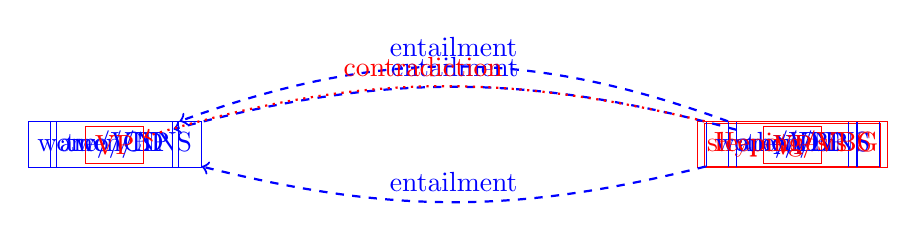
\begin{tikzpicture}[scale=0.7]
\begin{scope}[frontier/.style={distance from root=120pt}]
\Tree[.{Premise S} [.NP \node[draw,color=blue](p1){two/CD}; \node[draw,color=blue](p2){women/NNS}; ] [.VP \node[draw,color=blue](p3){are/VBP}; [.\node[draw,color=red](p4){VP}; hugging/VBG [.NP one/CD another/DT ] ] ] ]
\end{scope}
\begin{scope}[xshift=350pt,frontier/.style={distance from root=120pt}]
\Tree[.\node[draw,color=red]{Hypothesis S}; [.\node[draw,color=blue]{NP}; \node[draw,color=blue](h1){the/DT}; \node[draw,color=blue](h2){women/NNS}; ] [.\node[draw,color=red]{VP}; \node[draw,color=blue](h3){are/VBP}; \node[draw,color=red](h4){sleeping/VBG}; ] ]
\end{scope}

\begin{scope}[dashed]
\draw[thick,->,color=blue] (h1) to [bend right=15] node[above] {entailment}  (p1);
\draw[thick,->,color=blue] (h2) to [bend left=14] node[above] {entailment}  (p2);
\draw[thick,->,color=blue] (h3) to [bend right=20] node[above] {entailment}  (p3);
\draw[thick,dotted,->,color=red] (h4) to [bend right=15] node[above] {contradiction}  (p4);
\end{scope}
\end{tikzpicture}
\end{center}
\caption{Exemplary trees for the premise sentence 
``two women are hugging one another'' and 
the hypothesis sentence ``the women are sleeping''.
The syntactic labels (NP, VP, CD, etc.) are not used in the model.
The dashed and dotted lines show the lowest level of 
alignments from the hypothesis tree nodes
to the premise tree nodes.
The blue dashed lines mark the entailment relations,
and the red dotted line marks the contradiction relation.
In the hypothesis tree, tree nodes in blue squares
are identified to be entailment from the premise,
and nodes in red squared are identified to contradicts
the premise.
By composing these relations from the bottom up,
we reach a conclusion that the sentence-level entailment
relation is contradiction.
Please also refer to Figure~\ref{fig:ent-example}
for real examples taken from our experiments.
\label{fig:egtree}}
\end{figure*}